\chapter{Análisis de los Componentes Principales}

\section{¿Qué es el PCA?}
El \textbf{análisis de componentes principales} (\textit{Principal Component Analysis} - PCA) es una herramienta eficaz que ayuda a descubrir estructuras ocultas en grandes conjuntos de datos. Examina los datos complejos y multidimensionales para encontrar las perspectivas que nos den la mayor cantidad de información sobre los datos. Resalta los patrones más importantes y reduce aquellos menos importantes. El objetivo de PCA es reducir la dimensionalidad de los datos; ayuda a simplificar los datos en un conjunto más pequeño denominado «de componentes principales».


La varianza de los datos es como la diversidad de información. Una varianza alta es un indicador de que tiene una amplia gama de valores, lo que posiblemente indica una fuente rica en información. Entonces, PCA lo que hace es buscar direcciones donde esa variación sea máxima. Para elegir el primer componente principal, se intenta representar en una variable la mayor varianza posible. El segundo componente es independiente del primero; captura al igual que el primero la mayor varianza posible. Y así se crea cada uno de los componentes.

\section{Estructura matemática de PCA}
El algoritmo de PCA sigue los siguientes pasos:

\begin{enumerate}
    \item \textbf{Estandarización de datos} para garantizar que todas las características tengan la misma importancia.

    \item \textbf{Matriz de covarianza}: Es una matriz cuadrada que describe la variabilidad conjunta de dos variables. La matriz de covarianza es como una tabla que responde a la pregunta cuando una variable aumenta, ¿qué sucede con las demás? Los valores positivos indican una relación positiva (es decir, aumentan juntos), los valores negativos indican una relación negativa y cero indica que no hay relación.

    \item \textbf{Cálculo de valores y vectores propios}. Los \textbf{valores propios} (\textbf{eigenvalues}): indica cuánto estira o encoge un vector cuando se aplica una transformación lineal representada por una matriz. Los \textbf{vectores propios} (\textbf{eigenvectors}): son vectores que cuando se aplica una transformación lineal solo cambian en magnitud, no en dirección. Cada vector propio representa un componente. Lo interesante de estos vectores es que están orientados hacia donde los datos varían más.

    \item \textbf{Ordenar valores y vectores propios}. Para poder identificar los componentes principales, se deben ordenar los valores propios de forma descendente, de tal manera que mayor valor sea el primero de la lista.

    \item \textbf{Seleccionar los componentes principales}.  Se seleccionan los vectores propios con mayor valor propio. El primer componente principal corresponde al vector propio con el valor propio más grande, explicando la mayor varianza existente en el conjunto de datos. El segundo componente principal corresponde al vector propio con el segundo valor propio más grande, y así sucesivamente. El resultado es una matriz que proyecta los datos originales en un espacio de menor dimensión, reduciendo el conjunto de datos.
\end{enumerate}


\begin{figure}
    \centering
    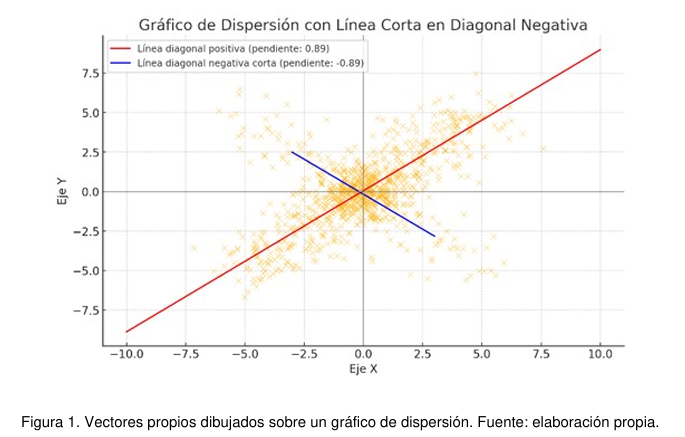
\includegraphics[width=0.5\linewidth]{imagenes/pca-grafico.png}

    \label{fig:pca-grafico}
\end{figure}


\section{Simplificación de datos}

PCA nos ofrece una solución elegante para controlar el problema de la maldición de la dimensionalidad. A medida que aumenta el número de dimensiones (características o variables) en un conjunto de datos, pueden ocurrir varios fenómenos complejos: escasez de datos, es decir, los puntos de datos tienden a estar más dispersos y para mantener la misma densidad, se necesitarían más datos; \textbf{grandes distancias entre datos} (la distancia entre puntos de datos tiende a aumentar y las diferencias entre las distancias se vuelven menos pronunciadas); la\textbf{ relevancia de las variables no es la misma}, ya que muchas puede que sean ruidosas o irrelevantes; \textbf{problemas computacionales} debido al procesamiento de datos con muchas dimensiones.


\section{Ventajas y casos de uso de PCA}
\begin{itemize}
    \item \textbf{Reducción de dimensionalidad}: al reducir el número de variables, los modelos se vuelven más simples.

    \item \textbf{Eliminación de redundancia}: ayuda a eliminar la multicolinealidad al transformar las variables originales en un nuevo conjunto de variables independientes.

    \item \textbf{Visualización en 2D y 3D}: facilita la visualización de datos complejos en dos o tres dimensiones.

    \item \textbf{Reducción de ruido}: al enfocarse en las componentes principales que captura la mayor varianza, deja de lado los componentes que representan ruido en el conjunto de datos.
\end{itemize}

Casos de uso:

\begin{itemize}
    \item \textbf{Compresión de imágenes}: al reducir la dimensionalidad de las imágenes y preservar su esencia, se pueden almacenar y transferir las imágenes.

    \item \textbf{Bioinformática}: las expresiones genéticas suelen ser conjuntos de datos de alta dimensionalidad, por lo que se puede aplicar PCA para identificar patrones y reducir el ruido. 

    \item \textbf{Reconocimiento facial}: permite la extracción de rasgos faciales esenciales para tareas de reconocimiento.

    \item \textbf{Sistemas de recomendación}: usar PCA suele obtener recomendaciones muy eficientes en datos de interacción entre un usuario y elementos en particular.
\end{itemize}

\section{Evaluación y mejora de PCA}
Existen algunos métodos para determinar el valor óptimo para el parámetro del número de componentes. Se puede realizar a través de dos visualizaciones diferentes. La primera solución es \textbf{graficar el porcentaje de varianza explicada} de los componentes individuales y el porcentaje de varianza total que capturan todos los componentes principales.

\begin{figure}[ht]
    \centering
    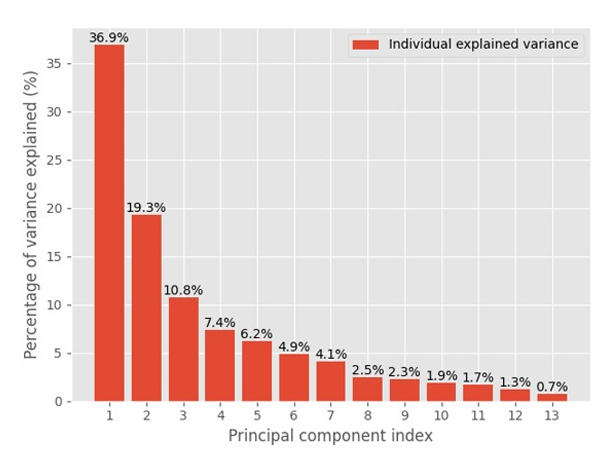
\includegraphics[width=0.75\linewidth]{imagenes/pca-grafica1.png}
    \label{fig:pca-grafica1}
\end{figure}

La segunda visualización es utilizar la técnica del codo utilizando el porcentaje de varianza explicada frente al número de componentes principales. Para poder decidir cuál es el número de componentes principales ideal.

\begin{figure}
    \centering
    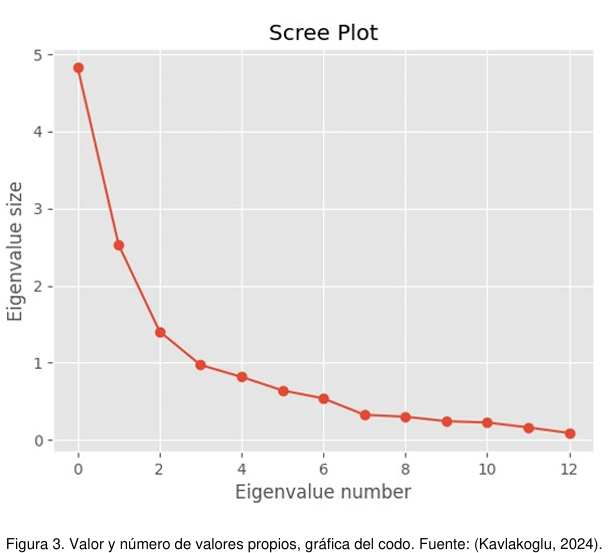
\includegraphics[width=0.75\linewidth]{imagenes/pca-grafica2.png}
    \label{fig:pca-grafica2}
\end{figure}